\documentclass{article}

\usepackage{graphicx} % Required for inserting images
\usepackage[T1]{fontenc}
\usepackage[utf8]{inputenc}
\usepackage[english]{babel}

\title{Dokumentacja Projektu Bazy danych 2 \\ \large Inwentaryzacja Sprzętu SKN MOS }

\author{Jakub Maciocha nr. albumu 272949 \and Kornel Uriasz nr. albumu 272967 \and Maciej Pacholczyk nr. albumu 272873}
\date{Październik 2024}

\begin{document}

\maketitle

\newpage
\section{\textbf{ETAP I - Opis świata rzeczywistego}}
    \subsection{Kontekst bieżący}
    Studenckie koło naukowego Microsystem Oriented Society (SKN MOS) prowadzi inwentaryzacje oraz możliwość wypożyczania sprzętu oraz narzędzi dla członków grupy w ramach działania koła naukowego. Siedziba koła zlokalizowana jest w podpiwniczeniu akademika T4 "Czworak", gdzie magazynowany jest sprzęt. Działanie opiera się na rejestrowaniu oraz monitorowaniu sprzętu oraz narzędzi przez administratorów koła naukowego. W tym przypadku są to członkowie zarządu. Katalogują oraz przechowując wszystkie informacje, które są im niezbędne do poprawnego działania koła oraz działania w ramach instytucji Politechniki Wrocławskiej. Taki system w bieżącym momencie pozwala w łatwy sposób zarządzać dostępnymi zasobami.

    \subsection{Opis zasobów ludzkich oraz procesów}
    Proces inwentaryzacji, na moment definiowania nowego systemu, opiera się na fizycznym odnotowywaniu nowego sprzętu z wykorzystanie numerów id lub jego nazwy. Archiwizacja urządzeń odbywa się w formie papierowej, na papierowym arkuszu. Spis sprzętów wypożyczonych prowadzony jest w oddzielnych zasobach w postaci listy  wypożyczeń. Lista ta jest przechowywana również na arkuszu papieru. Proces inwentaryzacji musi być jawny dla klienta jak i dla administratora tj. Klient musi wiedzieć co wypożyczyl i do kiedy musi oddać, administrator musi mieć jawną listę kto co ma, i kiedy ma oddać. Nie może nastąpić sytuacja, kiedy administrator nie wie gdzie jest dany przemiot, jak i nie może wystapić sytuacja, kiedy klient nie wie co ma wypożyczone i do kiedy ma to oddać.
    
    Inwentaryzacja w bieżącym momencie jest prosta, intuicyjna oraz łatwa do przyswojenia dla nowych członków koła, którzy systematycznie dołączają. Proces jest jednak mało wydajny przy zwiększającej się liczbie sprzętu oraz członków koła naukowego. Wzrost ilości dokumentacji dot. sprzętu oraz jego wypożyczeń skutkuje brakiem przejrzystości, trudnościami w archiwizacji oraz lokalizacją sprzętu. Podsumowując proces jest czasochłonny oraz podatny na błędy systemowe.

    W bieżącym momencie osoby działające w obrębie sytemu można podzielić na dwie grupy użytkowników. Pierwsza grupa to użytkownicy z uprawnieniami do odczytu. Klasyfikują się do niej członkowie koła, którzy mogą w swobodny sposób korzystać oraz wypożyczać sprzęt z placówki koła naukowego. W tym momencie do przedstawianego zbioru należy około \textbf{30} członków koła. Druga grupa użytkowników to administratorzy dbający o archiwizację oraz posiadający uprawnienia do wypożyczania sprzętu. Osoby
    te monitorują dostępne zasoby w kole naukowym oraz dbają o przechowywanie dokumentów potwierdzających stan odpowiednich przedmiotów. Do wymienionej grupy należy od \textbf{5 do 10} członków zarządu, którzy stają się administratorami. \newline
    Liczba administratorow : \textbf{5 - 10} \newline
    Liczba klientow : \textbf{30}
    
    Obciążenie serwera jest maksymalnie 10 zapytań na minute, w najgorszym przypadku, w najlepszym jest to 1 zapytanie na godzine.
\section{\textbf{ETAP II}}
    \subsection{Wymagania funkcjonalne i niefunkcjonalne}
    Klient (administratorzy) przedstawili następne funkcjonalności dla systemu usprawniającego proces inwentaryzacji oraz wypożyczeń.
        \begin{enumerate}
            \item Funkcjonalne
            
            \begin{enumerate}
                \item Aplikacja przedluża okres wypożyczenia na życzenie klienta, po zatwierdzeniu przez administratora
                \item Aplikacja ponagla o oddanie przedmiotu na zapytanie administratora
                \item Aplikacja decyduje o prawidłowym/nieprawidłowym oddaniu przedmiotu na podstawie daty wypożyczenia oraz aktualnej daty
                \item Aplikacja pokazuje przefiltrowane dane na żądanie klienta
                \item Aplikacja weryfikuje uprawnienia klienta
                \item Aplikacja wysyła powiadomienia o upływającym terminie wypożyczeń
                \item Aplikacja generuje miesięczne raporty sprzętowe
            \end{enumerate}

            \item Niefunkcjonalne 

            \begin{enumerate}
                \item Lokalizacja serwera w pokoju socjalnym w siedzibie koła naukowego
                \item Strona posiada przejrzysty interfejs
                \item Strona jest atrakcyjna/estetyczna
                \item Aplikacja jest umieszczona na serwerze koła naukowego
                \item Aplikacja przestrzega obostrzeń RODO
            \end{enumerate}
            
        \end{enumerate}

Diagram przypadkow uzycnia

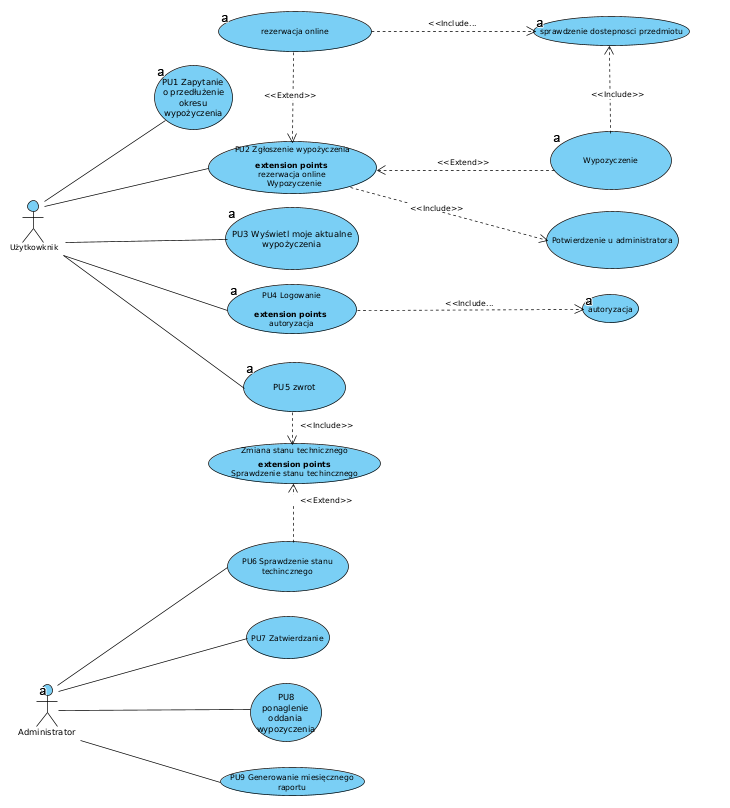
\includegraphics[width=\textwidth]{media/use_case.png}
\subsection{PU1: Rezerwacja}

\subsubsection{Cel}
Umożliwienie użytkownikowi zarezerwowania przedmiotu dostępnego w systemie na wybrany okres.

\subsubsection{Aktorzy}
\begin{itemize}
    \item \textbf{Użytkownik} - osoba korzystająca z systemu, która chce zarezerwować przedmiot.
\end{itemize}

\subsubsection{Zdarzenie inicjujące}
Użytkownik chce zarezerwować przedmiot, aby mieć pewność, że będzie on dostępny w określonym czasie.

\subsubsection{Warunki wstępne}
Użytkownik jest zalogowany do systemu i przedmiot, który chce zarezerwować, jest dostępny do rezerwacji.

\subsubsection{Warunki końcowe (wyniki)}
\begin{itemize}
    \item \textbf{Sukces:} Przedmiot jest zarezerwowany dla użytkownika na określony okres.
    \item \textbf{Niepowodzenie:} Użytkownik otrzymuje informację, że rezerwacja nie jest możliwa, ponieważ przedmiot nie jest dostępny.
\end{itemize}

\subsubsection{Scenariusz główny}
\begin{enumerate}
    \item Użytkownik loguje się do systemu.
    \item Użytkownik wybiera opcję „Rezerwacja” i przegląda dostępne przedmioty.
    \item Użytkownik wybiera przedmiot i określa termin, na który chce go zarezerwować.
    \item System sprawdza dostępność przedmiotu w wybranym terminie.
    \item Jeśli przedmiot jest dostępny, system rejestruje rezerwację.
    \item Użytkownik otrzymuje potwierdzenie rezerwacji.
\end{enumerate}

% Przypadek użycia 2: Wypożyczenie
\subsection{PU2: Wypożyczenie}

\subsubsection{Cel}
Umożliwienie użytkownikowi wypożyczenia przedmiotu na określony czas.

\subsubsection{Aktorzy}
\begin{itemize}
    \item \textbf{Użytkownik} - osoba korzystająca z systemu, która chce wypożyczyć przedmiot.
    \item \textbf{Administrator} - osoba odpowiedzialna za potwierdzenie wypożyczenia.
\end{itemize}

\subsubsection{Zdarzenie inicjujące}
Użytkownik chce wypożyczyć przedmiot na określony czas.

\subsubsection{Warunki wstępne}
Użytkownik jest zalogowany do systemu i przedmiot, który chce wypożyczyć, jest dostępny.

\subsubsection{Warunki końcowe (wyniki)}
\begin{itemize}
    \item \textbf{Sukces:} Przedmiot zostaje wypożyczony na rzecz użytkownika.
    \item \textbf{Niepowodzenie:} Użytkownik otrzymuje informację, że wypożyczenie nie jest możliwe (np. z powodu niedostępności przedmiotu).
\end{itemize}

\subsubsection{Scenariusz główny}
\begin{enumerate}
    \item Użytkownik loguje się do systemu.
    \item Użytkownik wybiera opcję „Wypożyczenie” i przegląda dostępne przedmioty.
    \item Użytkownik wybiera przedmiot do wypożyczenia i określa czas wypożyczenia.
    \item System sprawdza, czy przedmiot jest dostępny w wybranym czasie.
    \item Użytkownik potwierdza wypożyczenie.
    \item System przesyła prośbę do Administratora o potwierdzenie wypożyczenia.
    \item Administrator zatwierdza lub odrzuca wypożyczenie.
    \item Użytkownik otrzymuje informację o decyzji Administratora.
\end{enumerate}

% Przypadek użycia 3: Zwrot
\subsection{PU3: Zwrot}

\subsubsection{Cel}
Umożliwienie użytkownikowi zwrócenia wypożyczonego przedmiotu po zakończeniu okresu wypożyczenia.

\subsubsection{Aktorzy}
\begin{itemize}
    \item \textbf{Użytkownik} - osoba korzystająca z systemu, która chce zwrócić przedmiot.
    \item \textbf{Administrator} - osoba odpowiedzialna za sprawdzenie stanu technicznego zwróconego przedmiotu.
\end{itemize}

\subsubsection{Zdarzenie inicjujące}
Użytkownik kończy korzystanie z przedmiotu i chce go zwrócić.

\subsubsection{Warunki wstępne}
Użytkownik jest zalogowany do systemu i posiada wypożyczony przedmiot, który chce zwrócić.

\subsubsection{Warunki końcowe (wyniki)}
\begin{itemize}
    \item \textbf{Sukces:} Przedmiot zostaje zwrócony, a system aktualizuje jego stan jako dostępny.
    \item \textbf{Niepowodzenie:} Zwrot nie zostaje zrealizowany z powodu błędu w systemie lub problemu z przedmiotem.
\end{itemize}

\subsubsection{Scenariusz główny}
\begin{enumerate}
    \item Użytkownik loguje się do systemu.
    \item Użytkownik wybiera opcję „Zwrot” i wybiera przedmiot, który chce zwrócić.
    \item Użytkownik potwierdza zwrot przedmiotu.
    \item System rejestruje próbę zwrotu i informuje Administratora.
    \item Administrator sprawdza stan techniczny przedmiotu.
    \item Jeśli przedmiot jest w dobrym stanie, Administrator zatwierdza zwrot.
    \item System aktualizuje stan przedmiotu jako dostępny.
    \item Użytkownik otrzymuje potwierdzenie pomyślnego zwrotu.
\end{enumerate}

\section{\textbf{ETAP III}}

\subsection{\textbf{Diagramy ERD}}
  \begin{itemize}
    \item Konceptualny 
          Diagram konceptualny ERD (z ang. Entity-Relationship Diagram) przedstawia ogólną strukturę bazy danych, bez wnikania w szczegóły techniczne. Skupia się na identyfikacji kluczowych encji i ich relacji, aby zrozumieć, jakie informacje będą przechowywane w bazie i jak poszczególne elementy będą się ze sobą łączyć. Zostały w nim przedstawione tabele dostępne w systemie, relacje pomiędzy tabelami oraz kolumny zaiwerające klucz główny dla tabeli.   
    
    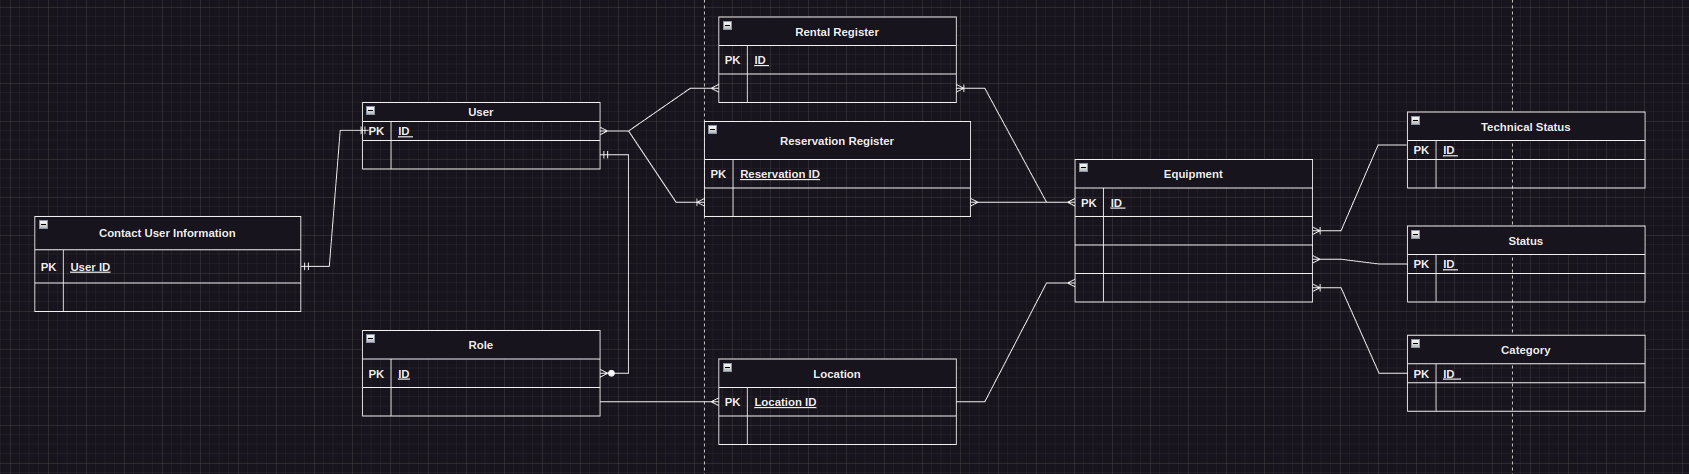
\includegraphics[width=\textwidth]{media/conceptual_erd.png}

    \item Logiczny
          Diagram logiczny ERD rozszerza konceptualny model danych, dodając szczegóły na temat struktur encji. Na tym etapie diagram przedstawia już kolumny z nazwami. Diagram logiczny pokazuje też typy relacji między encjami, w tym relacje wiele-do-wielu, jednak nadal pomija szczegóły techniczne związane z fizycznym implementowaniem bazy danych. Na diagramie pojawia się również typy kolumn w formie ogólnej, ale są one jeszcze niezwiązane z konkretnym silnikiem bazy danych.

     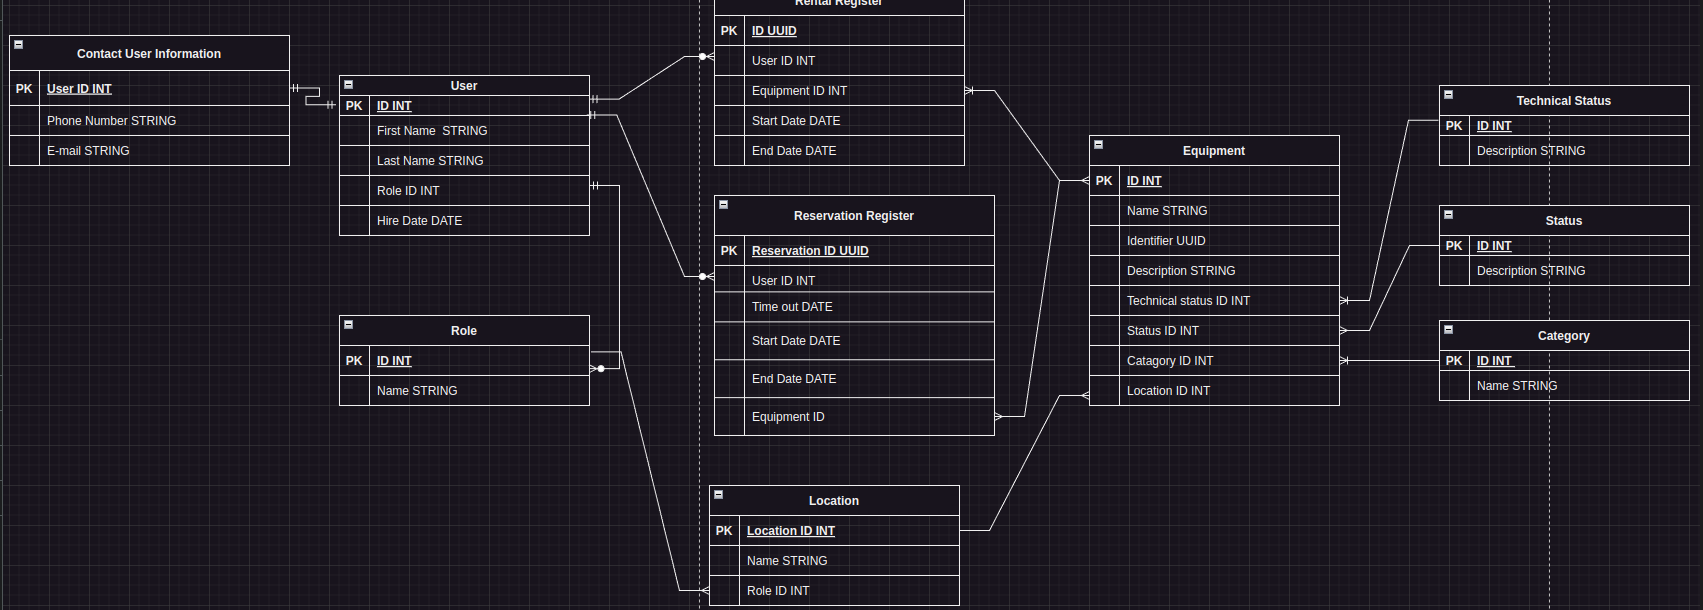
\includegraphics[width=\textwidth]{media/logical_erd.png}

    \item Fizyczny
        Diagram fizyczny ERD jest ostatecznym, szczegółowym modelem bazy danych, który uwzględnia wszystkie techniczne aspekty jej implementacji. Ten diagram zawiera wszystkie encje, kolumny oraz szczegółowe typy danych zgodne z wymaganiami wybranego silnika bazy danych. Nazwy encji i kolumn są dostosowane tak, aby były zgodne z konwencjami bazy danych (bez spacji i niedozwolonych znaków). Fizyczny ERD przedstawia także klucze główne oraz obce, a także rozwiązane relacje wiele-do-wielu, które są realizowane przez tabele pośredniczące. Diagram zwiera również  wyzwalacze (triggers) oraz inne mechanizmy logiczne potrzebne do poprawnego działania bazy danych.

      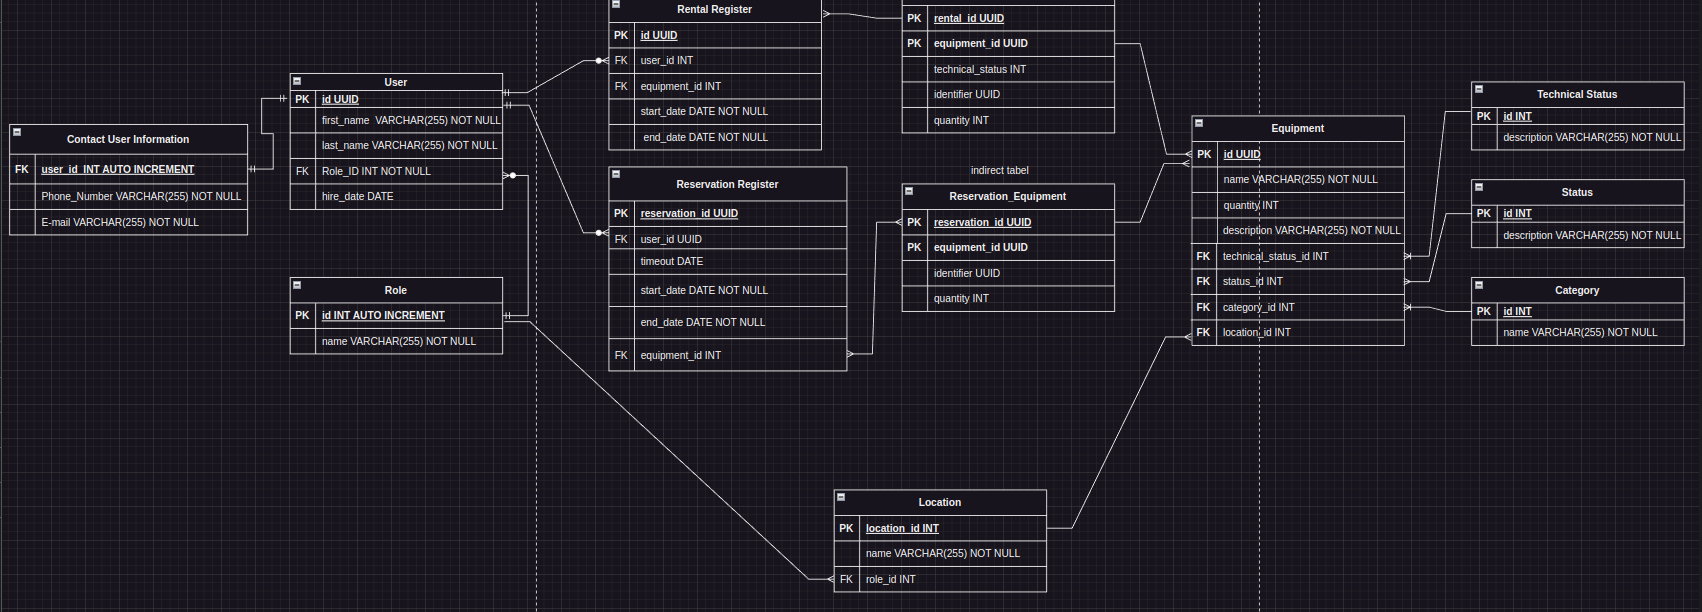
\includegraphics[width=\textwidth]{media/physical_erd.png}

  \end{itemize}

\subsection{\textbf{Analiza wielkości tabel i częstości odwołań do tabel i kolumn}}

Zakładając, że w systemie mamy \textbf{200 unikalnych przedmiotów (sprzętu)} oraz że liczba wypożyczeń wynosi \textbf{5 wypożyczeń tygodniowo}, poniżej przedstawiona jest analiza liczby rekordów w tabelach oraz częstości odwołań do tabel i kolumn.

\subsubsection{Liczność rekordów w tabelach}
Zakładając 5 wypożyczeń tygodniowo i średnio 2 przedmioty na wypożyczenie, liczba rekordów w tabelach wygląda następująco:

\begin{table}[h!]
    \centering
        \begin{tabular}{|l|l|l|}
            \hline
            \textbf{Tabela} & \textbf{Opis}  & \textbf{Liczba rekordów} \\ \hline
            Rental\_register & Rejestr wypożyczeń & 260 wypożyczeń rocznie \\ \hline
            Equipment & Lista sprzętu(200 unikalnych przedmiotów) & 200 rekordów \\ \hline
            Rental\_Equipment & Powiązania sprzętu z wypożyczeniami & 500 powiązań rocznie \\ \hline
        \end{tabular}
    \caption{Liczność rekordów w tabelach}
\end{table}

\subsubsection{\textbf{Częstość odwołań do tabel i kolumn}}
Poniżej przedstawiono przewidywaną częstość odwołań do tabel i kolumn na podstawie liczby operacji w systemie.

\begin{table}[h!]
    \centering
        \begin{tabular}[width=\textwidth]{|l|l|p{5cm}|l|}
            \hline
            \textbf{Tabela} & \textbf{Operacja} & \textbf{Opis} & \textbf{Częstość} \\ \hline
            Rental\_register& INSERT  & Dodawanie nowych wypożyczeń. & Niska  \\ \hline
             ~ & SELECT & Pobieranie historii wypożyczeń użytkowników. & Średnia. \\ \hline
             ~ & UPDATE & Aktualizacja dat zakończenia wypożyczeń lub innych danych. & Niska \\ \hline
            Equipment & SELECT & Pobieranie listy sprzętu. & Wysoka  \\ \hline
              & UPDATE & Zmiana statusu sprzętu. & Średnia \\ \hline
            Rental\_Equipment & SELECT & Pobieranie sprzętu dla danego wypożyczenia. & Średnia \\ \hline
              & INSERT & Dodawanie powiązań między wypożyczeniem a sprzętem. & Niska \\ \hline
        \end{tabular}
    \caption{Częstość odwołań do tabel i kolumn}
\end{table}

\subsubsection{Propozycje indeksów}
W celu optymalizacji zapytań, zwłaszcza dla tabel, które będą miały dużą liczbę operacji odczytu, zaproponowane indeksy wyglądają następująco:

\begin{itemize}
    \item \textbf{Tabela `Rental\_register`}: 
    \begin{itemize}
        \item \textbf{Primary Key:} `id` – identyfikator wypożyczenia.
        \item \textbf{Indeks:} `user\_id` – przyspiesza wyszukiwanie wypożyczeń dla konkretnego użytkownika.
        \item \textbf{Indeks:} `(start\_date, end\_date)` – ułatwia filtrowanie wypożyczeń w zadanym zakresie dat.
        \item \textbf{Indeks:} `equipment\_id` – umożliwia szybkie wyszukiwanie powiązań z poszczególnymi przedmiotami.
    \end{itemize}
    
    \item \textbf{Tabela `Equipment`}: 
    \begin{itemize}
        \item \textbf{Primary Key:} `id` – identyfikator sprzętu.
        \item \textbf{Indeks:} `status` – przyspiesza filtrowanie sprzętu według jego statusu (`available`, `rented`).
        \item \textbf{Indeks:} `category\_id` – przyspiesza filtrowanie sprzętu według kategorii.
    \end{itemize}
    
    \item \textbf{Tabela `Rental\_Equipment`}: 
    \begin{itemize}
        \item \textbf{Composite Primary Key:} `(rental\_id, equipment\_id)` – pozwala szybko łączyć dane z tabeli `Rental\_register` i `Equipment`.
        \item \textbf{Indeks:} `equipment\_id` – umożliwia szybkie wyszukiwanie sprzętu wypożyczonego w ramach danego wypożyczenia.
    \end{itemize}
\end{itemize}

\subsubsection{\textbf {Przykłady zapytań i ich optymalizacja}}

Poniżej przedstawiono przykłady zapytań oraz optymalizacje na podstawie proponowanych indeksów:

\begin{itemize}
    \item \textbf{Wyszukiwanie historii wypożyczeń użytkownika:}
    \begin{verbatim}
    SELECT * 
    FROM Rental_register 
    WHERE user_id = 123 
    ORDER BY start_date DESC;
    \end{verbatim}
    Indeks: `user\_id` oraz `(user\_id, start\_date)`.

    \item \textbf{Pobieranie dostępnego sprzętu w danej kategorii:}
    \begin{verbatim}
    SELECT * 
    FROM Equipment 
    WHERE status = 'available' AND category_id = 3;
    \end{verbatim}
    Indeks: `(status, category\_id)`.

    \item \textbf{Pobieranie sprzętu wypożyczonego w ramach danego wypożyczenia:}
    \begin{verbatim}
    SELECT e.name, e.description
    FROM Rental_Equipment re
    JOIN Equipment e ON re.equipment_id = e.id
    WHERE re.rental_id = 456;
    \end{verbatim}
    Indeks: `(rental\_id, equipment\_id)` w tabeli `Rental\_Equipment`.
\end{itemize}

\subsubsection{Podsumowanie}
Zmniejszenie liczby unikalnych przedmiotów (200 unikalnych przedmiotów) nie zmienia istotnie analizowanej struktury, jednak wpływa na zapytania przetwarzające dane o sprzęcie. Dla tabeli \texttt{Equipment}, która zawiera 200 rekordów, konieczne jest zastosowanie indeksów na kolumnach takich jak \texttt{status}, \texttt{category\_id} czy \texttt{id}, aby przyspieszyć operacje odczytu. Proponowane indeksy dla tabel \texttt{Rental\_register} i \texttt{Rental\_Equipment} powinny również zoptymalizować operacje wyszukiwania powiązań między wypożyczeniami a sprzętem.

Zoptymalizowane zapytania oraz odpowiednio zaplanowane indeksy zapewnią płynność działania systemu, nawet przy większej liczbie operacji odczytu i zapisu, co jest szczególnie istotne dla użytkowników oraz administratorów systemu.

\subsection{Analiza Integralności Danych}

Aby zapewnić integralność danych na podstawie dostarczonego diagramu ERD, analizujemy kluczowe zależności i relacje między tabelami. W poniższej tabeli przedstawiono rekomendowane akcje ``cascade delete'' lub wyzwalacze, które należy zastosować:

\begin{table}[h!]
    \centering
    \begin{tabular}{|p{4cm}|p{4cm}|p{6cm}|}
        \hline
        \textbf{Tabela źródłowa} & \textbf{Tabela zależna} & \textbf{Zalecana akcja} \\
        \hline
        User & Contact User Information & ON DELETE CASCADE \\
        \hline
        User & Rental Register & ON DELETE CASCADE \\
        \hline
        User & Reservation Register & ON DELETE CASCADE \\
        \hline
        Equipment & Rental Equipment & ON DELETE CASCADE \\
        \hline
        Equipment & Reservation Equipment & ON DELETE CASCADE \\
        \hline
        Technical Status, Status & Equipment & Wyzwalacz przed usunięciem \\
        \hline
    \end{tabular}
\end{table}

\subsubsection{Szczegóły}

\begin{itemize}
    \item \textbf{User $\rightarrow$ Contact User Information}: Klucz obcy z \texttt{user\_id} powinien mieć ``ON DELETE CASCADE'', aby po usunięciu użytkownika automatycznie usunąć powiązane dane kontaktowe.
    \item \textbf{User $\rightarrow$ Rental Register i Reservation Register}: Podobnie, po usunięciu użytkownika jego rekordy w tabelach rejestrów wynajmu i rezerwacji powinny również zostać usunięte.
    \item \textbf{Equipment $\rightarrow$ Rental Equipment i Reservation Equipment}: Usunięcie sprzętu powinno skutkować usunięciem powiązanych wypożyczeń i rezerwacji sprzętu.
    \item \textbf{Technical Status, Status $\rightarrow$ Equipment}: Wyzwalacz, który zapobiega usunięciu statusu, jeśli jest powiązany z istniejącym sprzętem.
    \item \textbf{Aktualizacja statusu sprzętu}: Wyzwalacz \texttt{AFTER UPDATE} w tabelach \texttt{Rental Register} i \texttt{Reservation Register} do automatycznego aktualizowania statusu sprzętu.
\end{itemize}

\subsection{Analiza Bezpieczeństwa i Poufności Danych}

Poniższa analiza dotyczy przypisania odpowiednich ról oraz poziomów dostępu do tabel w bazie danych, aby zapewnić bezpieczeństwo i poufność danych.

\subsubsection{Role i Zakres Uprawnień}

\begin{itemize}
    \item \textbf{Administrator}: Pełna kontrola nad całą bazą danych (SELECT, INSERT, UPDATE, DELETE, CREATE, ALTER, DROP).
    \item \textbf{Zarząd}: Dostęp do danych związanych z rejestracją użytkowników, rezerwacjami, wynajmem oraz sprzętem. Może dodawać, modyfikować i usuwać informacje o rejestracjach, ale bez dostępu do zarządzania użytkownikami.
    \item \textbf{MOSowicz}: Przeglądanie informacji o dostępności sprzętu, rezerwacjach i statusach technicznych. Może aktualizować stan techniczny sprzętu.
    \item \textbf{Rekrut}: Ograniczony dostęp do przeglądania sprzętu oraz tworzenia rezerwacji.
\end{itemize}

\subsubsection{Przypisanie Ról do Tabel i Uprawnień}

\begin{table}[!htbp]
\centering
    \begin{tabular}{|p{2cm}|p{2cm}|p{2cm}|p{2cm}|p{2cm}|}
        \hline
        \textbf{Tabela} & \textbf{Admin} & \textbf{Zarząd} & \textbf{MOSowicz} & \textbf{Rekrut} \\
        \hline
        User & SELECT, INSERT, UPDATE, DELETE & SELECT & Brak dostępu & Brak dostępu \\
        \hline
        Contact User Information & SELECT, INSERT, UPDATE, DELETE & Brak dostępu & Brak dostępu & Brak dostępu \\
        \hline
        Rental Register & SELECT, INSERT, UPDATE, DELETE & SELECT, INSERT, UPDATE, DELETE & SELECT & Brak dostępu \\
        \hline
        Reservation Register & SELECT, INSERT, UPDATE, DELETE & SELECT, INSERT, UPDATE, DELETE & SELECT & SELECT, INSERT \\
        \hline
        Rental Equipment & SELECT, INSERT, UPDATE, DELETE & SELECT, INSERT, UPDATE, DELETE & SELECT & Brak dostępu \\
        \hline
        Reservation Equipment & SELECT, INSERT, UPDATE, DELETE & SELECT, INSERT, UPDATE, DELETE & SELECT & SELECT \\
        \hline
        Equipment & SELECT, INSERT, UPDATE, DELETE & SELECT, INSERT, UPDATE & SELECT & SELECT \\
        \hline
        Technical Status & SELECT, INSERT, UPDATE, DELETE & SELECT, INSERT, UPDATE & SELECT, UPDATE & Brak dostępu \\
        \hline
        Status & SELECT, INSERT, UPDATE, DELETE & SELECT & SELECT & SELECT \\
        \hline
        Category & SELECT, INSERT, UPDATE, DELETE & SELECT, INSERT & Brak dostępu & Brak dostępu \\
        \hline
        Location & SELECT, INSERT, UPDATE, DELETE & SELECT, INSERT & SELECT & SELECT \\
        \hline
        Role & SELECT, INSERT, UPDATE, DELETE & Brak dostępu & Brak dostępu & Brak dostępu \\
        \hline
    \end{tabular}
\end{table}

\subsubsection{Dodatkowe Uwagi}

\begin{itemize}
    \item \textbf{Audyt i logowanie operacji}: Zaleca się wprowadzenie logowania dla operacji modyfikujących dane (INSERT, UPDATE, DELETE) w tabelach wrażliwych, takich jak \texttt{User} i \texttt{Rental Register}.
    \item \textbf{Szyfrowanie danych wrażliwych}: Dane osobowe, takie jak numer telefonu i e-mail, powinny być przechowywane w zaszyfrowanej formie.
    \item \textbf{Wyzwalacze kontroli dostępu}: Wyzwalacze sprawdzające, czy modyfikacje są dokonywane przez uprawnione role.
    \item \textbf{Kontrola dostępu oparta na roli (RBAC)}: Implementacja RBAC w celu ograniczenia dostępu do niezbędnych poziomów uprawnień.
\end{itemize}



\end{document}
